\documentclass[a4paper,11pt]{article}
%Przydatne paczki:
\usepackage{amssymb}
\usepackage{amsthm}
\usepackage{amsmath}
\usepackage[colorinlistoftodos]{todonotes}
\usepackage[colorlinks=true, allcolors=blue]{hyperref}
%Definicja kodowania i języka:
\usepackage[polish]{babel}
\usepackage[MeX]{polski}
\usepackage[utf8]{inputenc}
\usepackage[T1]{fontenc}
%Paczki dodane w drodze pisania:
\usepackage{graphicx}
\usepackage{anysize}
\selectlanguage{polish}
\usepackage{tabularx}
\usepackage[export]{adjustbox}
\usepackage{listings}
\usepackage{float}
\usepackage{fancyhdr}

%Nagłówek:
\pagestyle{fancy}
\fancyhead{}
\fancyhead[L]{\small{\bfseries \thepage}}
\fancyfoot[L, C, R] {}
\fancyhead[C]{\small{\bfseries Dokumentacja projektu "Reflekto"}}
\renewcommand{\headrulewidth}{0.8pt}

%\marginsize{left}{right}{top}{bottom}
\marginsize{2.5cm}{2.5cm}{2.5cm}{2.5cm}

\begin{document}

\title{Dokumentacja projektu \\ \textbf{,,Reflekto'' } }
\author{Michał Kwiecień \\ Michał Wójcik}
%skomentować żeby nie było daty
%\date{\vspace{-5ex}}
\maketitle

\begin{abstract}
Dokumentacja projektu inteligentnego lustra w konwencji IoT komunikującego się ze smartfonem z użyciem interfejsu Bluetooth Low Energy. Projekt powstał na potrzeby konkursu Nordic Semiconductor Student Contest. 
\end{abstract}

\begin{figure}
	
\includegraphics[width=0.3\textwidth,center]{logo_nordic.png}
\end{figure}

\cleardoublepage
\tableofcontents
\clearpage

\section{Ogólny opis projektu}

Założeniem projektu jest stworzenie inteligentnego lustra, które podczas wykonywania codziennych czynności, umożliwi podgląd najświeższych i spersonalizowanych informacji. Informacje te zostaną wyświetlone na ekranie umieszczonym za lustrem weneckim, dzięki czemu będą widoczne jednocześnie obok odbicia. 

Działanie lustra opiera się na przekazaniu danych poprzez moduł Bluetooth ze smartfona do modułu nRF52 i umieszczeniu ich na podłączonym ekranie. Aktywacja lustra nastąpi w momencie zbliżenia się do niego użytkownika. Z lustra może korzystać wielu użytkowników, gdyż każdorazowo przesyłane są indywidualne dane dla każdego z nich. 

W celu wygenerowania danych stworzona została dedykowana aplikacja dla systemu iOS. Po wstępnej konfiguracji umożliwi ona zautomatyzowanie procesu i przesyłanie wiadomości w tle bez późniejszych ingerencji użytkownika.


\section{Prezentacja działania}

Kiedy lustro nie jest w bliskim zasięgu jednego ze sparowanych telefonów, wyświetlana jest godzina lub pozostaje wyłączone w zależności od ustawień (Rys. \ref{lustro_off})

\begin{figure}[H]
	
\includegraphics[width=0.6\textwidth,center]{mirror_off.png}
	\caption {Lustro w stanie wyłączonym}
	\label{lustro_off}
\end{figure}

W momencie zbliżenia się użytkownika, następuje transmisja danych i wyświetlenie aktualnych wiadomości (Rys. \ref{lustro_on}).

\begin{figure}[H]
	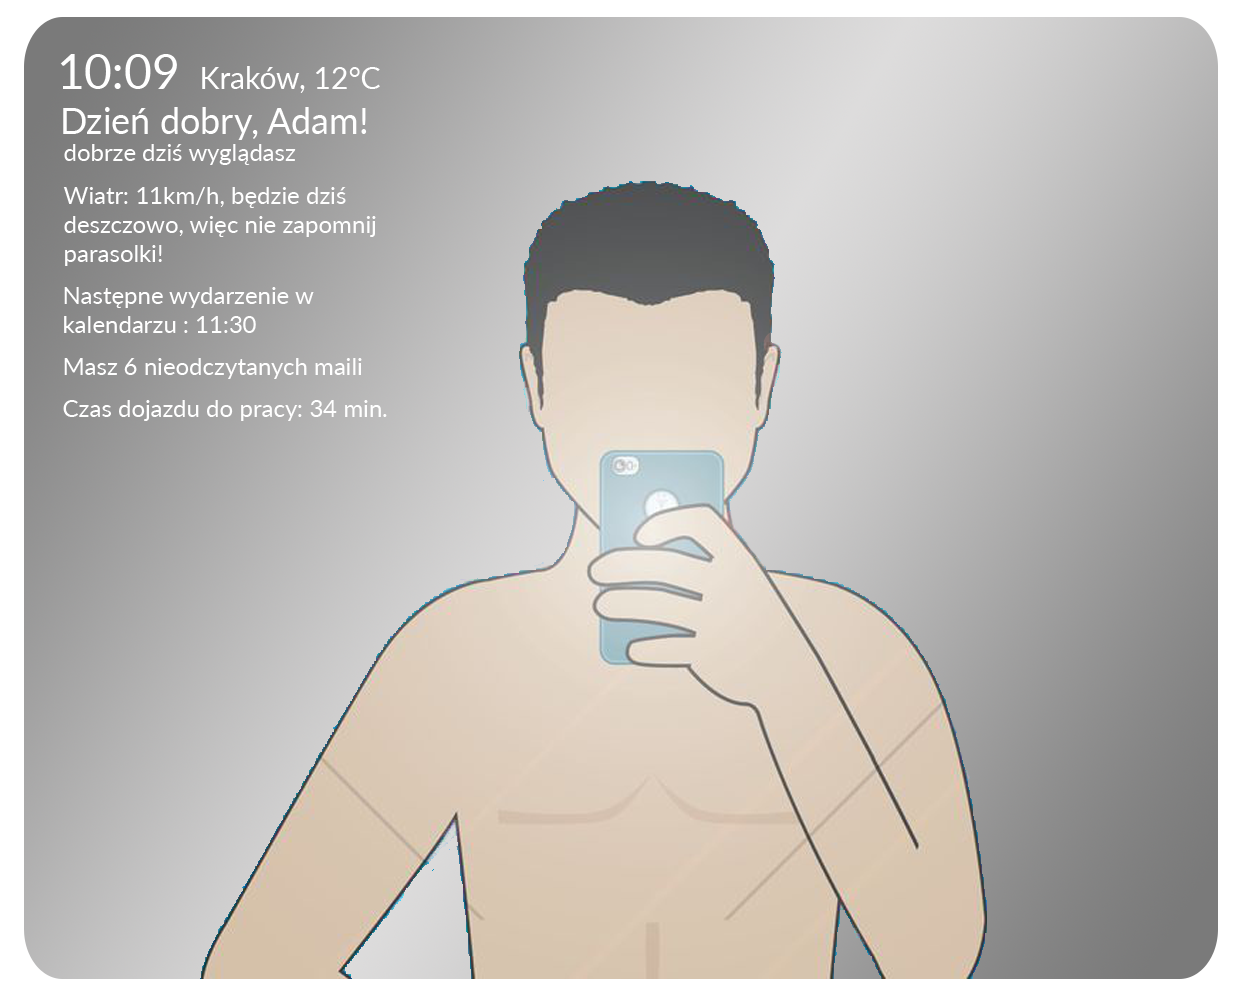
\includegraphics[width=0.6\textwidth,center]{mirror_on.png}
	\caption {Lustro w stanie aktywnym}
	\label{lustro_on}
\end{figure}

\section{Planowane możliwości personalizacji}
\begin{figure}[H]
	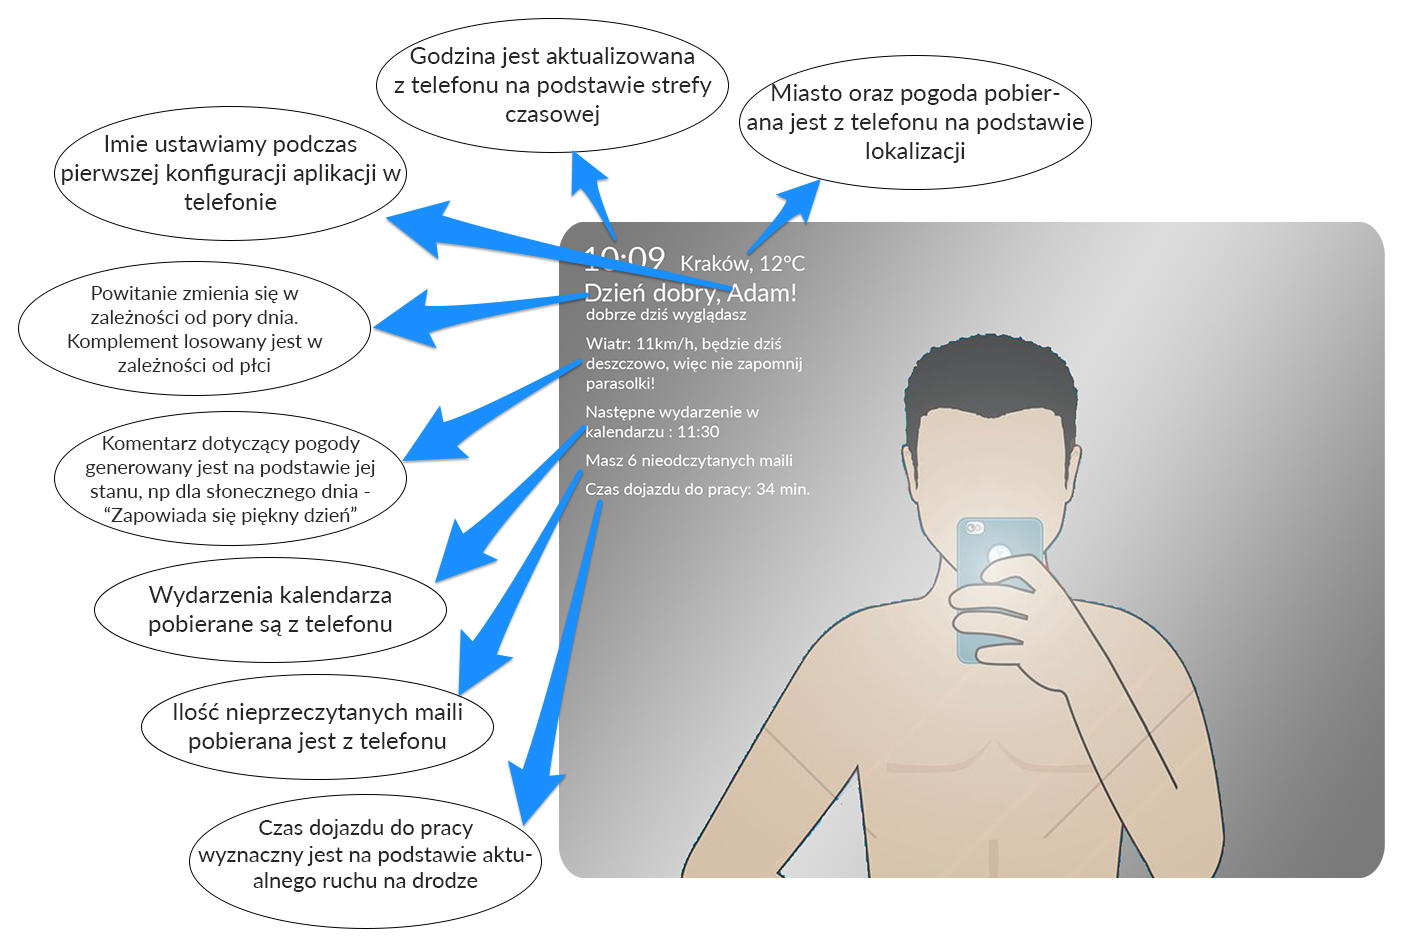
\includegraphics[width=0.9\textwidth,center]{dymki_kreski.png}
	\caption {Proponowane możlwości personalizacji}
	\label{lustro_on}
\end{figure}

\section{Opis aplikacji systemu nRF52 (stan na 9 kwietnia 2017) }

\subsection{Włączenie urządzenia}
Urządzenie po uruchomieniu inicjalizuje wszystkie niezbędne usługi: timer, uart, stos BLE, serwisy oraz obsługę wyświetlacza. Dalej rozpoczyna się rozgłaszanie (pod nazwą ,,Reflekto\_UART'') i urządzenie pozostaje w stanie oczekiwania aż do wyłączenia zasilania. 
\subsection{Zasilanie}
Ze względu na użycie wyświetlacza TFT, wymagane jest zasilanie przez zasilacz zewnętrzny bądź port USB (bateria pastylkowa nie pokrywa zapotrzebowania na prąd). Obecnie szacowany pobór energii w stanie aktywnym wynosi mniej niż 1W. W stanie nieaktywnym pobór energii przez wyświetlacz może zostać zredukowany do zera (sterowanie PWM), jednakże wymaga to wlutowania odpowiedniej zworki w płytkę wyświetlacza.

\subsection{Sposób rozgłaszania}
Do urządzenia w tym samym czasie może być podłączony jeden smartfon. W zależności od ustawień, 
 może być on połączony do momentu zachowania bliskiego zasięgu (potencjalnie blokując innych użytkowników), \todo{Możliwe korzystanie przez kilku użytkowników jednocześnie} 
lub rozłączać się od razu po przesłaniu informacji. 

Układ rozgłasza się pod wcześniej zdefiniowaną nazwą i UUID, udostępniając jeden serwis, z charakterystyką ,,write'' oraz ,notify'' (obecnie niewykorzystana).

\subsection{Realizacja komunikacji}
Układ w momencie otrzymania danych wysyła je do komputera przez port szeregowy (w celu debugowania), oraz rzutuje je na wektor typu \textit{char}, który przekazywany jest do kolejnej funkcji realizującej umieszczenie danych na wyświetlaczu.

Ze względu na ograniczenie ilości danych w pakiecie do 20 bajtów zastosowano specjalne kodowanie, gdzie pierwsze dwa bajty analizowane są w następujący sposób: 
\begin{itemize}
	\item bajt ,,0''
	\subitem Wskazuje na typ otrzymanych danych (np. data, godzina, pogoda, kalendarz, e-mali) \todo{4 bity można użyć do ,,szyfrowania'' transmisji}
	\item bajt ,,1''
	\subitem 4 bity górne -- numer aktualnie otrzymanego pakietu
	\subitem 4 bity dolne -- ilość wszystkich pakietów danego typu
\end{itemize}
Wynika z tego maksymalna długość przesyłanych danych jednego typu do 288 znaków. Podział na paczki realizowany jest przez aplikację na smartfonie. Założono takżę obsługę błędnych pakietów przez SoftDevice'a, dlatego nie uwzględnione zostały bajty na sumę CRC.

\subsection{Umieszczanie informacji na wyświetlaczu}
Po otrzymaniu wszystkich paczek danego typu, dane ,,drukowane'' są na wyświetlaczu (ze względu na metodę komunikacji niemożliwe jest przesłanie jednorazowo całej ramki obrazu). Wyświetlacz podzielony został na sekcje (od góry):
\begin{itemize}
	\item 20\% -- aktualna data i godzina
	\item 20\% -- aktualna pogoda
	\item 60\% -- kalendarz, czas dojazdu do pracy, emaile itd. wyświetlane cyklicznie bądź jednocześnie
\end{itemize}

\subsection{Konfiguracja}
W planach jest obsługa danych konfiguracyjnych, które ustalałyby np. sposób wyświetlania informacji, lub działania układu w trybie niekatywnym.
\section{Opis aplikacji systemu iOS (stan na 9 kwietnia 2017)}



	
\end{document}